\documentclass[12pt]{article}
\usepackage{amsmath}
\usepackage{graphicx}
\usepackage{hyperref}
\usepackage{listings}
\usepackage{color}
\usepackage{float}

\lstset{
    language=Python,                      % Set bahasa ke Python
    basicstyle=\ttfamily\footnotesize,    % Ukuran dan font kode
    keywordstyle=\color{blue},            % Warna keyword
    stringstyle=\color{red},              % Warna string
    commentstyle=\color{green},           % Warna komentar
    numbers=left,                         % Menampilkan nomor baris
    numberstyle=\tiny,                    % Ukuran nomor baris
    stepnumber=1,                         % Setiap baris diberi nomor
    breaklines=true,                      % Pemenggalan baris otomatis
    frame=single,                         % Bingkai di sekitar kode
    tabsize=4                             % Ukuran tab
}

\title{Operating System Course Report - First Half of the Semester}
\author{B class}
\date{\today}

\begin{document}

\maketitle
\newpage

\tableofcontents
\newpage

\section{Introduction}
This report summarizes the topics covered during the first half of the Operating System course. It includes theoretical concepts, practical implementations, and assignments. The course focuses on the fundamentals of operating systems, including system architecture, process management, CPU scheduling, and deadlock handling.

\section{Course Overview}
\subsection{Objectives}
The main objectives of this course are:
\begin{itemize}
    \item To understand the basic components and architecture of a computer system.
    \item To learn process management, scheduling, and inter-process communication.
    \item To explore file systems, input/output management, and virtualization.
    \item To study the prevention and handling of deadlocks in operating systems.
\end{itemize}

\subsection{Course Structure}
The course is divided into two halves. This report focuses on the first half, which covers:
\begin{itemize}
    \item Basic Concepts and Components of Computer Systems
    \item System Performance and Metrics
    \item System Architecture of Computer Systems
    \item Process Description and Control
    \item Scheduling Algorithms
    \item Process Creation and Termination
    \item Introduction to Threads
    \item File Systems
    \item Input and Output Management
    \item Deadlock Introduction and Prevention
    \item User Interface Management
    \item Virtualization in Operating Systems
\end{itemize}

\section{Topics Covered}

\subsection{Basic Concepts and Components of Computer Systems}
This section explains the fundamental components that make up a computer system, including the CPU, memory, storage, and input/output devices.

\subsection{System Performance and Metrics}
\subsubsection{\textit{Performance Metrics} Pada \textit{CPU}}
\hspace*{1cm} Jika kita membahas kinerja matriks pada komputer, maka kita tidak bisa lepas dari CPU. CPU atau \textit{Central Processing Unit} adalah komponen utama dari komputer yang bertanggung jawab mengeksekusi instruksi-instruksi yang diberikan kepada komputer. Kinerja suatu sistem sangat dipengaruhi oleh cara CPU mengeksekusi instruksi. Untuk memaksimalkan kinerja suatu sistem, kita tentu perlu meminimalkan waktu eksekusi, karena kinerja berbanding terbalik dengan waktu eksekusi.
\newline
\newline
\hspace*{1cm} Untuk menentukan waktu eksekusi CPU untuk suatu program, Anda dapat mencari tahu jumlah total \textit{\textit{clock} cycle} yang dibutuhkan program dan mengalikannya dengan waktu \textit{\textit{clock} cycle}. Setiap program terdiri dari sejumlah instruksi, dan setiap instruksi membutuhkan sejumlah \textit{\textit{clock} cycle} untuk dieksekusi. Jika Anda mengetahui jumlah total \textit{\textit{clock} cycle} per program serta mengetahui waktu \textit{\textit{clock} cycle} untuk setiap \textit{\textit{clock} cycle}, maka waktu eksekusi CPU dapat dihitung sebagai hasil perkalian jumlah total \textit{\textit{clock} cycle} CPU per program dengan waktu \textit{\textit{clock} cycle}. Karena waktu \textit{\textit{clock} cycle} dan \textit{\textit{clock} rate} saling terkait, hal ini juga dapat ditulis sebagai jumlah \textit{\textit{clock} cycle} CPU untuk suatu program dibagi dengan \textit{\textit{clock} rate}.

\begin{figure}
    \centering
    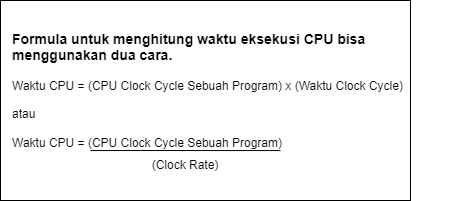
\includegraphics[width=\linewidth]{asset/image1.png}
    \caption{Rumus waktu CPU}
\end{figure}


\hspace*{1cm} Karena waktu eksekusi CPU merupakan hasil dari kedua faktor ini, kita dapat meningkatkan kinerja dengan mengurangi durasi waktu \textit{clock cycle} atau jumlah \textit{clock cycle} yang diperlukan untuk suatu program. Kecepatan \textit{clock} pada dasarnya bergantung pada organisasi CPU tertentu.

\subsubsection{Mengapa \textit{Performance Metrics} Penting}
\hspace*{1cm} Mengukur kinerja menggunakan data yang akurat sangat penting dalam sebuah sistem karena memberikan gambaran nyata tentang performa yang sedang berlangsung. Dengan data yang tepat, manajemen dapat membuat keputusan yang lebih terinformasi, sehingga memperkecil risiko kesalahan dalam strategi. Selain itu, pengukuran kinerja juga membantu mengidentifikasi area yang memerlukan perbaikan, sehingga organisasi dapat berfokus pada peningkatan yang signifikan. Memantau perkembangan dan kemajuan kinerja secara berkala meningkatkan akuntabilitas, baik di tingkat individu maupun tim, sehingga setiap anggota lebih bertanggung jawab atas hasil kerjanya. Pada akhirnya, penggunaan \textit{performance metrics} yang tepat dapat mendorong peningkatan berkelanjutan dengan memberikan dasar yang kuat untuk evaluasi dan inovasi secara sistematis dalam mencapai tujuan jangka panjang.

\subsubsection{Fungsi \textit{Performance Metrics} pada Sistem}
\hspace*{1cm} \textit{Performance metrics} berperan penting dalam berbagai aspek sistem operasi. Berikut adalah beberapa area di mana \textit{performance metrics} digunakan:
\begin{itemize}
    \item \textbf{\textit{Benchmark}} \newline
    \hspace*{1cm} \textit{Benchmark} biasanya menggunakan berbagai \textit{performance metrics} untuk mengukur dan melaporkan hasil kinerjanya. Misalnya, sebuah \textit{benchmark} untuk prosesor mungkin mengukur metrik seperti kecepatan \textit{clock}, jumlah instruksi per detik (\textit{IPS}), atau waktu komputasi untuk tugas tertentu.
    \item \textbf{\textit{Bandwidth}} \newline  
    \hspace*{1cm} Mengukur jumlah data yang dapat ditransmisikan melalui jaringan dalam jangka waktu tertentu. \textit{Bandwidth} yang terbatas membatasi kemampuan sistem untuk menangani banyak permintaan atau mentransfer data dalam jumlah besar, yang pada akhirnya memperlambat waktu muat atau respons. Pada sistem yang sangat bergantung pada transfer data, seperti aplikasi berbasis web atau layanan \textit{cloud}, \textit{bandwidth} adalah faktor penting yang memengaruhi performa keseluruhan.
    \item \textbf{\textit{Error Rate}} \newline  
    \hspace*{1cm} Menghitung persentase permintaan yang gagal diproses atau menghasilkan kesalahan. Metrik ini penting untuk menilai stabilitas dan keandalan sistem. Tingkat kesalahan yang tinggi menunjukkan masalah pada sistem, seperti bug dalam perangkat lunak, kesalahan konfigurasi, atau keterbatasan sumber daya. Tingkat kesalahan yang tinggi dapat mengganggu pengguna dan menurunkan kepercayaan mereka terhadap sistem.
    \item \textbf{Pengaturan Kualitas Layanan (\textit{QoS})} \newline  
    \hspace*{1cm} Dalam lingkungan yang membutuhkan kualitas layanan tertentu, \textit{performance metrics} digunakan untuk memastikan bahwa aplikasi dan layanan memenuhi \textit{SLA} (\textit{Service Level Agreement}). Metrik seperti latensi, \textit{throughput}, dan waktu respons digunakan untuk mengatur dan memantau \textit{QoS}.
    \item \textbf{Optimasi dan Tuning} \newline  
    \hspace*{1cm} \textit{Performance metrics} digunakan untuk mengidentifikasi peluang optimasi dan tuning. Misalnya, dengan
\end{itemize}

\hspace*{1cm} \textit{Performance metrics} berperan penting dalam berbagai aspek pengelolaan dan operasional sistem operasi. Dari monitoring dan manajemen sumber daya hingga optimasi, diagnosis, dan keamanan, metrik ini memberikan wawasan yang diperlukan untuk menjaga sistem tetap berjalan dengan efisien, aman, dan sesuai dengan kebutuhan kinerja yang diharapkan.

\subsection{System Architecture of Computer Systems}
Describes the architecture of modern computer systems, focusing on the interaction between hardware and the operating system.

\subsection{Process Description and Control}
Processes are a central concept in operating systems. This section covers:
\begin{itemize}
    \item Process states and state transitions
    \item Process control block (PCB)
    \item Context switching
\end{itemize}

\subsection{Scheduling Algorithms}
This section covers:
\begin{itemize}
    \item First-Come, First-Served (FCFS)
    \item Shortest Job Next (SJN)
    \item Round Robin (RR)
\end{itemize}
It explains how these algorithms are used to allocate CPU time to processes.

\subsection{Process Creation and Termination}
Details how processes are created and terminated by the operating system, including:
\begin{itemize}
    \item Process spawning
    \item Process termination conditions
\end{itemize}

\subsection{Introduction to Threads}
This section introduces the concept of threads and their relation to processes, covering:
\begin{itemize}
    \item Single-threaded vs. multi-threaded processes
    \item Benefits of multithreading
\end{itemize}

\subsection{File Systems}
File systems provide a way for the operating system to store, retrieve, and manage data. This section explains:
\begin{itemize}
    \item File system structure
    \item File access methods
    \item Directory management
\end{itemize}

\subsection{Input and Output Management}
Input and output management is key for handling the interaction between the system and external devices. This section includes:
\begin{itemize}
    \item Device drivers
    \item I/O scheduling
\end{itemize}

\subsection{Deadlock Introduction and Prevention}
Explores the concept of deadlocks and methods for preventing them:
\begin{itemize}
    \item Deadlock conditions
    \item Deadlock prevention techniques
\end{itemize}

\subsection{User Interface Management}
\subsubsection{Graphical User Interface (GUI)}
\subsubsection{Graphical User Interface (GUI)}
		
		GUI telah menjadi standar de facto untuk interaksi pengguna dalam sistem operasi modern. 
        GUI menyajikan informasi melalui elemen visual seperti ikon, menu, jendela, dan kontrol grafis lainnya, 
        memungkinkan pengguna untuk berinteraksi dengan komputer menggunakan perangkat penunjuk seperti mouse atau layar sentuh \cite{Shneiderman2016}.
		
		Komponen kunci GUI dalam sistem operasi modern meliputi:
		\begin{itemize}
			\item Desktop Environment: Menyediakan latar belakang kerja utama, termasuk wallpaper, ikon desktop, dan panel/dock.
			\item Window Manager: Mengontrol penempatan dan tampilan jendela aplikasi.
			\item Widget Toolkit: Menyediakan elemen UI standar seperti tombol, menu, dan kotak dialog.
			\item Compositing Manager: Menangani efek visual seperti transparansi dan animasi.
			\item Notification System: Mengelola dan menampilkan pemberitahuan sistem dan aplikasi.
		\end{itemize}
		
		GUI menawarkan beberapa keunggulan signifikan:
		\begin{itemize}
			\item Intuitivitas: Pengguna dapat dengan mudah memahami dan menggunakan sistem tanpa pelatihan ekstensif.
			\item Visualisasi: Informasi kompleks dapat disajikan dalam format yang mudah dipahami.
			\item Multitasking: Pengguna dapat dengan mudah beralih antara dan mengelola beberapa aplikasi secara bersamaan.
			\item Aksesibilitas: Fitur seperti pembaca layar dan pengaturan kontras tinggi dapat diintegrasikan untuk mendukung pengguna dengan kebutuhan khusus.
		\end{itemize}

		Perkembangan terbaru dalam GUI meliputi antarmuka adaptif yang menyesuaikan diri dengan konteks penggunaan dan preferensi pengguna, serta integrasi teknologi seperti pengenalan gestur dan kontrol suara \cite{Murad2021}.

\subsection{Virtualization in Operating Systems}
Virtualization allows multiple operating systems to run concurrently on a single physical machine. This section explores:
\begin{itemize}
    \item Concept of virtualization
    \item Hypervisors and their types
    \item Benefits of virtualization in modern computing
\end{itemize}


\section{Assignments and Practical Work}
\subsection{Assignment 1: Process Scheduling}
\hspace*{1cm} Implementasikan algoritma penjadwalan \textit{Shortest Job First} (SJF) dan \textit{Round Robin} (RR), lalu bandingkan rata-rata waktu tunggu (\textit{average waiting time}) dan rata-rata waktu penyelesaian (\textit{average turnaround time}) dari kedua algoritma tersebut. Manakah yang lebih baik dalam menangani proses? 
\newline
\newline

\begin{center}
    \underline{JAWABAN}
\end{center}

\textit{Short Job First (SJF) algorithms}
\begin{lstlisting}[language=Python]
    def sjf_non_preemptive(Jumlah_proses):
        Jumlah_proses.sort(key=lambda x: x[1])
    
        waktu_tunggu = 0
        total_waktu_tunggu = 0
    
        for pid, burst_time in Jumlah_proses:
            total_waktu_tunggu += waktu_tunggu
            waktu_tunggu += burst_time
    
        n = len(Jumlah_proses)
        avg_waktu_tunggu = total_waktu_tunggu / n
    
        print(total_waktu_tunggu)
        print(f"\nAverage Waiting Time: {avg_waktu_tunggu}")    
    
\end{lstlisting}

\textit{Round Robin (RR) algorithms}
\begin{lstlisting}[language=Python]
    def round_robin(jumlah_proses, quantum):
        n = len(jumlah_proses)
        remaining_time = [bt for _, bt in jumlah_proses]
        waktu_tunggu = [0] * n
        time = 0
    
        while True:
            done = True
            for i in range(n):
                if remaining_time[i] > 0:
                    done = False
                    if remaining_time[i] > quantum:
                        time += quantum
                        remaining_time[i] -= quantum
                    else:
                        time += remaining_time[i]
                        waktu_tunggu[i] = time - jumlah_proses[i][1]
                        remaining_time[i] = 0
            if done:
                break
    
        avg_waktu_tunggu = sum(waktu_tunggu) / n
        print(f"\nAverage Waiting Time: {avg_waktu_tunggu:.2f}")
    
\end{lstlisting}

\begin{figure}[H]
    \centering
    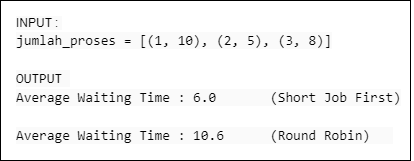
\includegraphics[width=1\linewidth]{asset/41.png}
    \caption{Output}
\end{figure}

\begin{figure}[H]
    \centering
    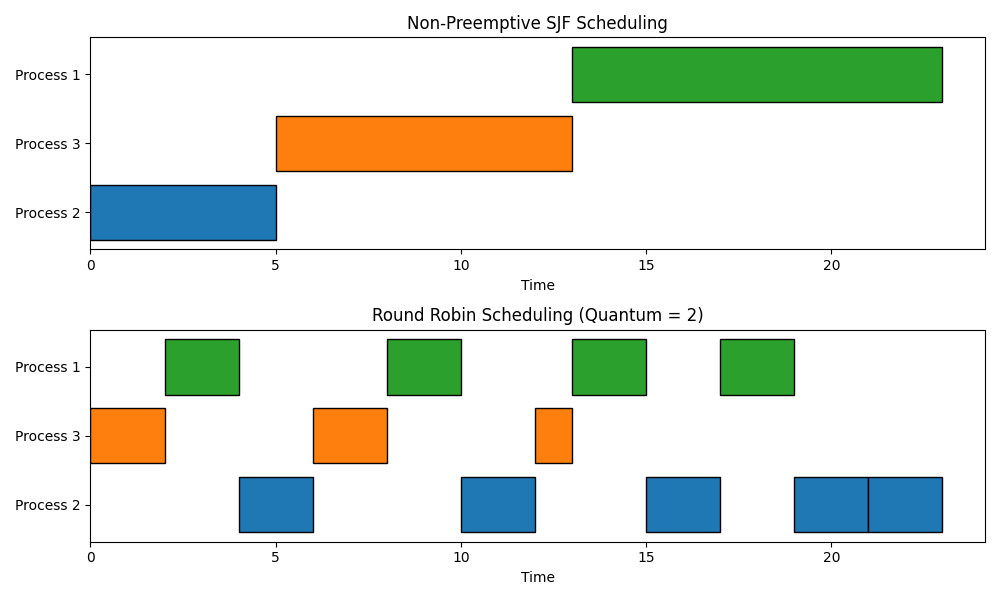
\includegraphics[width=1\linewidth]{asset/411.png}
    \caption{Perbandingan SJF dan RR(quantum = 2)}
\end{figure}

\paragraph{
    \hspace*{1cm} Dari hasil perbandingan rata-rata waktu tunggu pada kedua algoritma, dapat dilihat bahwa rata-rata waktu tunggu SJF lebih kecil dibandingkan dengan \textit{Round Robin}. Salah satu alasannya adalah karena sifat RR yang memberikan setiap proses sejumlah waktu yang sama (\textit{quantum}) dan memaksa semua proses menunggu giliran mereka secara bergantian. 
}

\paragraph{
    \hspace*{1cm} Kita dapat mengurangi kelemahan \textit{Round Robin} dengan memilih \textit{quantum} yang lebih besar. Pada visualisasi di atas terlihat bahwa waktu tunggu RR dapat sama dengan SJF. Namun, tetap saja, SJF sering kali lebih baik dalam kasus dengan banyak proses yang memiliki \textit{burst time} yang bervariasi.
}

\begin{figure}[H]
    \centering
    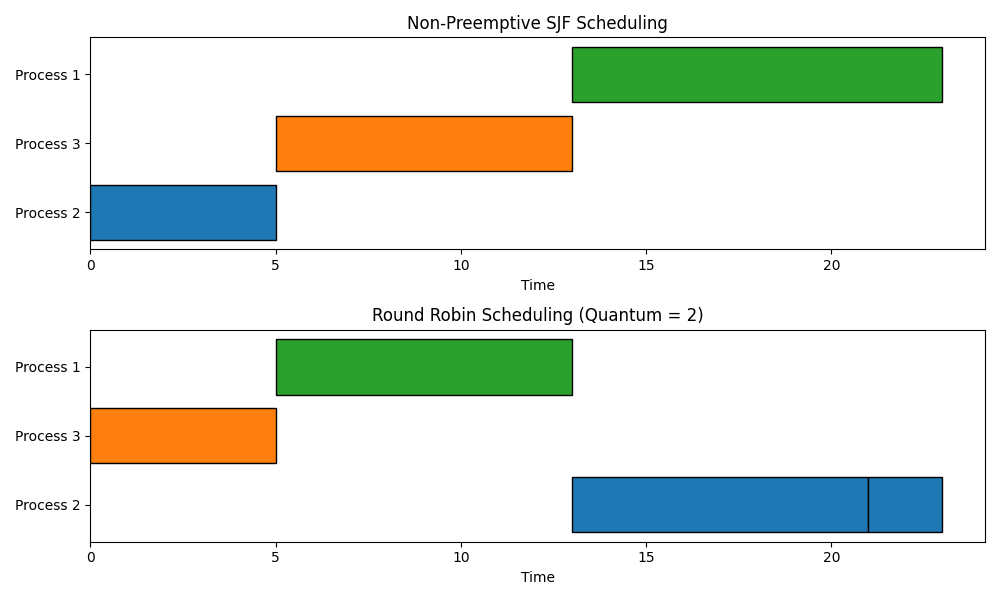
\includegraphics[width=1\linewidth]{asset/412.png}
    \caption{Perbandingan SJF dan RR(quantum = 8)}
\end{figure}


\subsection{Assignment 2: Deadlock Handling}
\hspace*{1cm} Simulasikan bagaimana \textit{algoritma safety} bekerja untuk mendeteksi \textit{deadlock}.
\newline
\newline

\begin{center}
    \underline{JAWABAN}
\end{center}

\begin{lstlisting}[language=Python]

    import numpy as np
    
    def is_safe(Jumlah_proses, avail, max_need, allocation):
        P, R = len(Jumlah_proses), len(avail) 
        need = max_need - allocation 
        finish = [False] * P 
        safe_sequence = []  
        work = avail.copy() 
    
        for _ in range(P):
            for p in range(P):
                if not finish[p] and all(need[p] <= work): 
                    work += allocation[p]
                    finish[p] = True
                    safe_sequence.append(p)
                    break
            else:
                print("Sistem tidak dalam keadaan aman.")
                return False, []
    
        print("Sistem dalam keadaan aman.")
        return True, safe_sequence
    
    
    Jumlah_proses = [0, 1, 2, 3, 4]
    avail = np.array([3, 3, 2]) 
    max_need = np.array([[7, 5, 3],
                         [3, 2, 2],
                         [9, 0, 2],
                         [2, 2, 2],
                         [4, 3, 3]]) 
    allocation = np.array([[0, 1, 0],
                           [2, 0, 0],
                           [3, 0, 2],
                           [2, 1, 1],
                           [0, 0, 2]]) 
    
    is_safe_state, safe_sequence = is_safe(Jumlah_proses, avail, max_need, allocation)
    
    if is_safe_state:
        print("Sistem dalam urutan aman:", safe_sequence)
    else:
        print("Tidak ada urutan aman, sistem dalam keadaan deadlock.")
    
\end{lstlisting}

\begin{figure}[H]
    \centering
    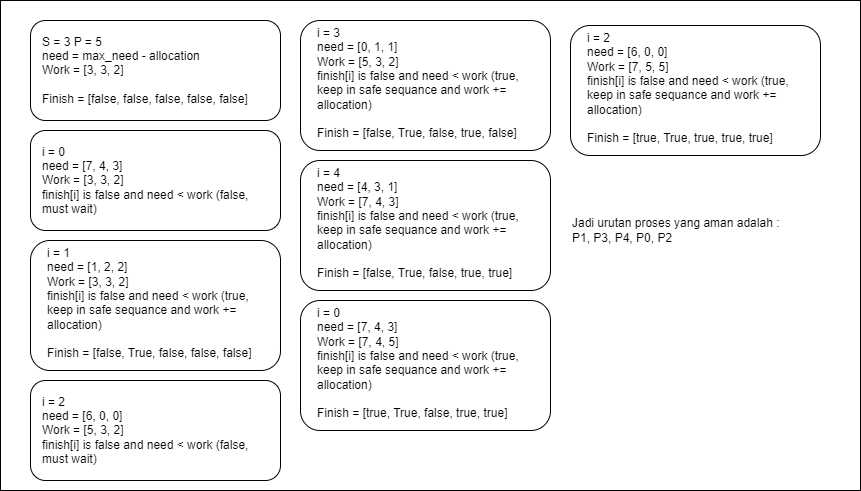
\includegraphics[width=1\linewidth]{asset/421.png}
    \caption{Output dan Penjelasannya}
\end{figure}

\paragraph{
    \hspace*{1cm} Dengan menggunakan metode \textit{Banker's} untuk algoritma \textit{Safety}, kita bisa memastikan bahwa sistem aman jika menjalankan proses-proses tertentu. Di sini, kita memeriksa setiap proses dan memastikan bahwa alokasi sumber daya untuk setiap proses dapat dilakukan dengan aman sehingga tidak akan menyebabkan \textit{deadlock}. Pada output, sistem akan menampilkan status apakah sistem aman atau tidak, dan menampilkan urutan proses yang aman.
}


\begin{python}
    import threading
    import time
    
    resource_a = threading.Lock()
    resource_b = threading.Lock()
    
    def process_1():
        print("Process 1: Acquiring Resource A")
        with resource_a:
            time.sleep(1)  
            print("Process 1: Acquiring Resource B")
            with resource_b:
                print("Process 1: Working with both resources")
    
    def process_2():
        print("Process 2: Acquiring Resource B")
        with resource_b:
            time.sleep(1)  
            print("Process 2: Acquiring Resource A")
            with resource_a:
                print("Process 2: Working with both resources")
    
    t1 = threading.Thread(target=process_1)
    t2 = threading.Thread(target=process_2)
    
    t1.start()
    t2.start()
    
    t1.join()
    t2.join()
    \end{python}
    
    To prevent deadlocks, we can ensure a consistent order of resource acquisition:
    
    \begin{python}
    def process_1():
        print("Process 1: Acquiring Resource A")
        with resource_a:
            time.sleep(1)  
            print("Process 1: Acquiring Resource B")
            with resource_b:
                print("Process 1: Working with both resources")
    
    def process_2():
        print("Process 2: Acquiring Resource A")
        with resource_a:
            time.sleep(1)  
            print("Process 2: Acquiring Resource B")
            with resource_b:
                print("Process 2: Working with both resources")
    
    
    t1 = threading.Thread(target=process_1)
    t2 = threading.Thread(target=process_2)
    
    
    t1.start()
    t2.start()
    
    t1.join()
    t2.join()
    \end{python}

\subsection{Assignment 3: Multithreading and Amdahl's Law}
\hspace*{1cm} Simulasikan skenario \textit{multithreading} untuk menghitung jumlah kuadrat dari rentang angka yang diberikan dan menjumlahkannya, dan terapkan \textit{Amdahl law} untuk menghitung prediksi kecepatan seiring penambahan \textit{thread} untuk mengetahui penggunaan jumlah \textit{thread} yang optimal.
\newline
\newline

\begin{center}
    \underline{JAWABAN}
\end{center}

\begin{lstlisting}[language=Python]

    import threading
    import time
    
    def compute_squares(start, end, results, index, execution_times):
        start_time = time.time()
        print(f"Thread {index} mulai menghitung dari {start} hingga {end}...")
        result = 0
        for number in range(start, end):
            time.sleep(0.0001) 
            result += number * number
        results[index] = result
        end_time = time.time()
        execution_times[index] = end_time - start_time
        print(f"Thread {index} selesai menghitung dalam {execution_times[index]:.4f} detik.")
    
    total_range = 10000
    num_threads = 4  
    step = total_range // num_threads
    
    
    results = [0] * num_threads
    execution_times = [0] * num_threads
    
    threads = []
    
    start_time = time.time()
    for i in range(num_threads):
        start = i * step
        end = (i + 1) * step if i != num_threads - 1 else total_range
        thread = threading.Thread(target=compute_squares, args=(start, end, results, i, execution_times))
        threads.append(thread)
        thread.start()
    
    for thread in threads:
        thread.join()
    end_time = time.time()
    
    total_execution_time = end_time - start_time
    total_result = sum(results)
    
    def amdahl_law(P, N):
        return 1 / ((1 - P) + (P / N))
    
    
    sequential_fraction = 0.1  
    P = 1 - sequential_fraction
    
    print("Semua thread selesai.")
    print(f"Hasil perhitungan: {total_result}")
    print(f"Waktu eksekusi total: {total_execution_time:.4f} detik")
    
    print("Speedup teoretis menurut Hukum Amdahl:")
    for N in range(1, num_threads + 1):  
        speedup = amdahl_law(P, N)
        print(f"Speedup teoretis dengan {N} thread: {speedup:.2f}x")
    
\end{lstlisting}

\begin{figure}[H]
    \centering
    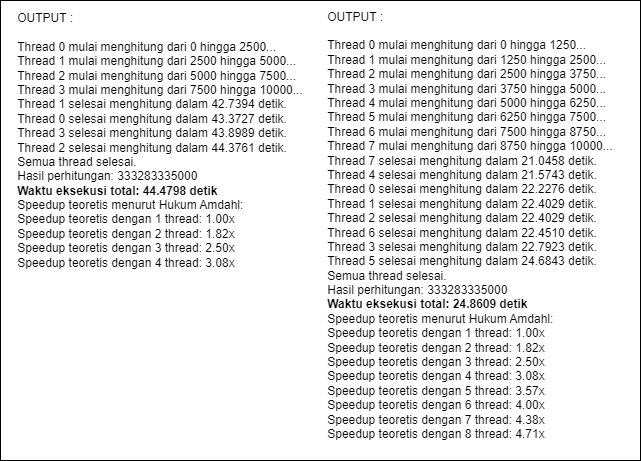
\includegraphics[width=1\linewidth]{asset/31.png}
    \caption{Eksekusi dengan 4 threads (kiri) dan eksekusi dengan 8 threads (kanan)}
\end{figure}

\paragraph{
    \hspace*{1cm} Pada algoritma di atas, \textit{multithreading} berfungsi untuk membagi proses berdasarkan jumlah \textit{thread} yang digunakan, sehingga kita bisa membuat waktu eksekusi menjadi lebih singkat. Dengan menggunakan algoritma \textit{Amdahl's Law}, kita bisa melihat rasio peningkatan kecepatan seiring meningkatnya jumlah \textit{thread} yang digunakan. Dapat dilihat pada perbedaan output di atas, bahwa dengan meningkatkan jumlah \textit{thread} dari 4 ke 8, waktu eksekusi juga meningkat.
}



\subsection{Assignment 4: Simple Command-Line Interface (CLI) for User Interface Management}
Students were tasked with creating a simple **CLI** for user interface management. The CLI should support basic commands such as file manipulation (creating, listing, and deleting files), process management, and system status reporting.

\subsection{Assignment 5: File System Access}
In this assignment, students implemented file system access routines, including:
\begin{itemize}
    \item File creation and deletion
    \item Reading from and writing to files
    \item Navigating directories and managing file permissions
\end{itemize}

\section{Conclusion}
The first half of the course introduced core operating system concepts, including process management, scheduling, multithreading, and file system access. These topics provided a foundation for more advanced topics to be covered in the second half of the course.

\begin{thebibliography}{9}
    \bibitem{gfg2024}
    TestingXperts. (2022, May 10). Performance testing metrics: A detailed guide for businesses. Digital Assurance. Retrieved October 8, 2024, from https://www.testingxperts.com
    \bibitem{gfg2024}
    GeeksforGeeks. (n.d.). Computer organization: Performance of computer. GeeksforGeeks. Retrieved October 1, 2024, from https://www.geeksforgeeks.org/computer-organization-performance-of-computer/
    \bibitem{gfg2024}
    GeeksforGeeks. (2024, August 20). Program for round robin scheduling for the same arrival time. GeeksforGeeks. Retrieved October 8, 2024, from https://www.geeksforgeeks.org/program-for-round-robin-scheduling-for-the-same-arrival-time/
\end{thebibliography}

\end{document}